\noindent
\begin{tabular}{cc}
\begin{minipage}{0.95\textwidth}
\begin{exerciseS}[Motore alternativo]
Il funzionamento di un motore alternativo a benzina (a quattro tempi) può essere rappresentato in prima approssimazione con un ciclo termodinamico Otto ideale, rappresentato da una compressione adiabatica, una fase veloce di combustione a volume costante (nel punto morto superiore del moto del pistone, PMS) e un'espansione adiabatica. Le fasi di aspirazione e scarico dei gas combusti sono anch'essi ideali. L'aspirazione avviene a pressione costante durante il movimento del pistone dal PMS al punto morto inferiore (PMI). La fase di scarico avviene in due fasi: durante la prima fase la pressione diminuisce molto velocemente (approssimata da una trasformazione a volume costante) a causa dell'apertura della valvola di scarico quando il pistone si trova al PMI; durante la seconda fase i gas combusti sono spinti fuori dalla camera di combustione dal movimento ascendente del pistone che si riporta al PMS, per l'inizio del ciclo termodinamico successivo. Del motore sono noti:
\begin{itemize}
 \item il rapporto di compressione, definito come il rapporto tra il volume massimo (pistone al PMI) e minimo (pistone al PMS) della camera di combustione, $r = V_1 / V_2 = 10$;
 \item la cilindrata, definita come la corsa del pistone per l'area della sezione del cilindro, e uguale alla differenza $C = N (V_2 - V_1) = 1000 \ cc$, essendo $N$ il numero di cilindri del motore;
 \item le condizioni termodinamiche dell'aria all'aspirazione $P_0 = 85570 \, Pa$, $T_0 = 25°C$;
 \item il rapporto in massa tra benzina e aria, $f = m_f / m_a = 0.06$;
 \item il potere calorifico della benzina usata $\Delta h = 43 \, MJ$;
 \item la pressione nel basamento del motore, $p_{b} = 150000 \, Pa$ uniforme e costante.
Si calcoli la potenza media erogata dal motore a un regime di rotazione di $\Omega = 3000 RPM$, assumendo un rendimento meccanico $\eta = 0.8$.
Si rappresenti l'aria come un gas bi-atomico perfetto ($\gamma = c_P/ c_v = 1.4$) con costante dei gas $R = 287 J / (kg \, K)$, e si trascuri l'effetto del carburante sul valore dei calori specifici e sulla massa presente all'interno della camera di combustione. Si trascurino inoltre gli scambi di calore per conduzione con l'esterno del cilindro durante la compressione e l'espansione (trasformazioni adiabatiche). Si trascurino i termini cinetici nell'energia totale in camera di combustione, facendo coincidere l'energia totale con l'energia interna $e^t = e = c_v T$, e si assuma che le variabili termodinamiche siano uniformi (costanti in spazio, non in tempo) in camera di combustione.
\end{itemize}
\end{exerciseS}
\end{minipage}
\end{tabular}
\begin{figure}[h]
 \centering
 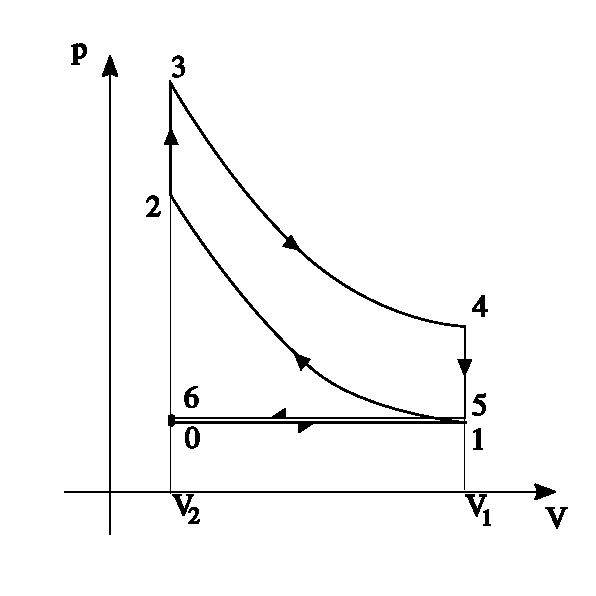
\includegraphics[width=0.45\textwidth]{./fig/otto_cycle}
\end{figure}

% todo: figure with the cut-out of the cylinder, thermodynamic cycle

%
\sol

% Concetti
\partone
Ogni fase del ciclo termodinamico viene analizzata con i bilanci integrali, per il volume corrispondente alla camera di combustione di un cilindro. Questo volume è un sistema aperto durante la fase di aspirazione e scarico (scambia massa con l'esterno), mentre è un sistema chiuso durante la compressione, la combustione e l'espansione (valvole chiuse, nessuno scambio di massa con l'esterno). Si calcola il lavoro svolto dal sistema durante un ciclo e si divide per il periodo per ricavare la potenza media. 

% Svolgimento
\parttwo
Conoscendo il numero dei cilindri $N=3$, il rapporto di compressione $r$ e la cilindrata $C$ è possibile ricavare il valore del volume massimo $V_1$ e minimo $V_2$ della camera di combustione.
\begin{equation}
\begin{cases}
 N( V_2 - V_1 ) = C \\
 V_1 / V_2 = r
\end{cases} \qquad \rightarrow \qquad
\begin{cases}
 V_1 = \dfrac{r}{r-1} \dfrac{C}{N} \\ \\ 
 V_2 = \dfrac{1}{r-1} \dfrac{C}{N}
\end{cases} 
\end{equation}
Si analizzano ora le fasi del ciclo termodinamico, fornendo una breve descrizione e ponendo attenzione allo scambio di massa (sistema chiuso/aperto), lavoro e calore con l'esterno.
\begin{itemize}
\item \textbf{Aspirazione}, $0 \rightarrow 1$: la prima fase del ciclo Otto è l'aspirazione. Durante la fase di aspirazione (ideale), la valvola di aspirazione è aperta e il sistema scambia massa con l'esterno: il pistone si sposta dal PMS al PMI e la camera di combustione si riempie d'aria a pressione e temperatura costante,
\begin{equation}
 p_1 = p_0 \qquad , \qquad
 T_1 = T_0 \qquad , \qquad
 \rho_1 = \rho_0 = \dfrac{p_0}{R T_0} =
\end{equation}
La massa contenuta nella camera di combustione alla chiusura della valvola, in coincidenza del PMI, è
\begin{equation}
 m = \rho_1 V_1 = \dots \ .
\end{equation}
Durante la fase di aspirazione, il pistone deve vincere la sovrapressione del basamento (di solito la pressione nel basamento è superiore a quella aspirata in camera di combustione). Dal PMS al PMI un pistone assorbe parte della potenza fornita dagli altri pistoni. Il lavoro che assorbe è $L_{01} = -(p_b-p_0) \, c$ (negativo poichè assorbito), essendo $c$ la corsa del pistone e la differenza di pressione costante durante l'aspirazione. Questo lavoro assorbito durante l'aspirazione sarà uguale e contrario a quello fornito durante lo scarico ideale dei gas,  che avviene alla stessa differenza di pressione con un moto opposto.
\item \textbf{Compressione}, $1 \rightarrow 2$: la seconda fase del ciclo termodinamico è la compressione del fluido che avviene a causa del movimento verso l'alto del pistone. Il sistema è chiuso: le valvole sono chiuse e si ipotizza che non ci sia trafilamento (\textit{blow-by}) tra il pistone e la superficie laterale del cilindro. Il bilancio di energia totale per il fluido contenuto all'interno del volume $V(t)$ (variabile nel tempo, a causa del moto del pistone) della camera di combustione,
\begin{equation}
 \dfrac{d}{dt} \displaystyle\int_{V(t)} \rho e^t + \oint_{S(t)} \rho e^t (\bm{u}-\bm{v}) \cdot \bm{\hat{n}}= \int_{V(t)} \bm{f} \cdot \bm{u} + \oint_{S(t)} \bm{t_n} \cdot \bm{u} - \oint_{S(t)} \bm{q} \cdot \bm{\hat{n}} + \int_{V(t)} \rho r \ .
\end{equation}
può essere semplificato, trascurando l'effetto delle forze di volume, $\bm{f} = \bm{0}$, trascurando la trasmissione del calore con l'esterno (trasformazione adiabatica), $\bm{q} \cdot \bm{\hat{n}} = 0$, e non essendoci sorgenti di calore, $r = 0$. Inoltre non c'è flusso di massa attraverso il contorno $S(t)$ del volume, $(\bm{u}-\bm{v}) \cdot \bm{\hat{n}} = 0$, e l'unica superficie in movimento della camera di combustione corrisponde al cielo (la faccia superiore) del pistone, $S_{c}$. Trascurando il contributo cinetico e approssimando l'energia totale $e^t = e + |\bm{u}|^2/2$ con l'energia interna $e$, il bilancio di energia diventa,
\begin{equation}
 \dfrac{d}{dt} \displaystyle\int_{V(t)} \rho e = \int_{S_c(t)} \bm{t_n} \cdot \bm{u} \ ,
\end{equation}
legando la derivata temporale dell'energia del fluido nella camera di combustione alla potenza delle forze esercitate dal pistone sul fluido. La potenza delle forze agenti sul pistone è uguale all'integrale superficiale del prodotto scalare vettore sforzo $\bm{t_{n,s}}$ agente sul solido per la velocità $\bm{v}$ della superficie del solido,
\begin{equation}
\begin{aligned}
 W_{12} = \oint_{S_{s}} \bm{t_{n,s}} \cdot \bm{v}
 & = \int_{S_{s,c}} \bm{t_{n,s}} \cdot \bm{v} + \int_{S_{s,b}} \bm{t_{n,s}} \cdot \bm{v}  + \int_{S_{s,lat}} \bm{t_{n,s}} \cdot \bm{v} = \\
 & = - \int_{S_{c}} \bm{t_{n}} \cdot \bm{u} - \int_{S_{s,b}} p_b\bm{\hat{n}_{s}} \cdot \bm{v} \ ,
\end{aligned}
\end{equation}
avendo suddiviso la superficie del cilindro $S_s$ come l'unione della superficie superiore $S_{s,c}$ (cielo), superficie laterale $S_{s,lat}$ (dal contributo nullo, per simmetria), e superifice inferiore $S_{s,b}$ esposta verso il basamento del motore, sulla quale agisce uno sforzo dovuto alla pressione $p_b$ dell'ambiente all'interno del basamento. \'E stato indicata con $\bm{\hat{n}_s}$ la normale uscente dalla superficie del solido e con $\bm{t_{n,s}}$ il vettore sforzo agente su un punto della superficie del solido, uguale e contrario a quello agente sul fluido $\bm{t_n} = -\bm{t_{n,s}}$ per il principio di azione e reazione. Inoltre, le condizioni al contorno impongono che il fluido e il solido abbiano la stessa velocità $\bm{u} = \bm{v}$ sulle superfici di contatto.
Si può quindi riscrivere il bilancio di energia del fluido in funzione della potenza $W_{12}$ trasmessa al pistone,
\begin{equation}
  \dfrac{d}{dt} \displaystyle\int_{V(t)} \rho e = - W_{12} - p_b S_{c} \ v(t) = - W_{12} - p_b \dfrac{d V}{d t} \ ,
\end{equation}
essendo $v(t)$ la velocità del pistone, per ottenere la potenza trasmessa al pistone dal fluido (sarà una potenza richiesta, $<0$),
\begin{equation}
\begin{aligned}
  W_{12}(t) & = - \dfrac{d}{dt} \displaystyle\int_{V(t)} \rho e - p_b \dfrac{d V}{d t} = \\
  & = - \dfrac{d}{dt} \left( \rho V e \right) - p_b \dfrac{d V}{d t} = \\
  & = - m \dfrac{d e}{d t} - p_b \dfrac{d V}{d t} \ ,
\end{aligned}
\end{equation}
nell'ipotesi di variabili termodinamiche uniformi nel volume, ricordando che la massa contenuta nella camera di combustione $m = \rho V$ rimane costante, essendo un sistema chiuso, se si trascura l'effetto di trafilamento tra le pareti di cilindro e pistone (ridotte al minimo da fasce elastiche e anelli raschiaolio sul pistone e sovra-pressione nel basamento).
\newline \noindent
Integrando in tempo la potenza istantantea $W_{12}(t)$, tra il punto 1 e il punto 2 del ciclo, si ottiene il lavoro di compressione
\begin{equation}
 L_{12} = - m (e_2 - e_1) - p_b ( V_2 - V_1 ) \ .
\end{equation}
Utilizzando la legge di stato dei gas perfetti $p = \rho R T$ e il legame tra le variabili termodinamiche durante una trasformazione adiabatica $p/\rho^\gamma = \text{cost}$, si ottiene
\begin{equation}
 e_2 - e_1 = c_v ( T_2 - T_1 ) = c_v T_1 \left[ \left( \dfrac{\rho_2}{\rho_1} \right)^{\gamma-1} - 1 \right] = c_v T_1 \left( r^{\gamma-1} - 1\right) \ .
\end{equation}

\item \textbf{Combustione}, $2 \rightarrow 3$: la terza fase del ciclo termodinamico è la combustione. Viene iniettato il combustibile all'interno della camera di combustione, innescata dall'accensione di una candela in un motore a benzina classico. Durante l'iniezione del combustibile il sistema è aperto. In prima approssimazione si può trascurare la variazione di massa, $m + m_f = m ( 1 + f ) \simeq m$. In prima approssimazione, si può rappresentare questa fase con una trasformazione isocora (volume costante) associata a un aumento di pressione e temperatura, a causa di una combustione (completa) veloce in corrispondenza del PMS. Il bilancio di energia che descrive questa fase diventa
\begin{equation}
\begin{aligned}
 \dfrac{d}{dt} \displaystyle\int_{V(t)} \rho e & = \int_{V(t)} \rho r \\
 m \dfrac{d e}{d t} & = \dot{m}_f \Delta h \qquad \rightarrow \qquad
 e_3 - e_2 = \dfrac{ m_f }{ m } \Delta h  = f \Delta h \ .
\end{aligned}
\end{equation}
Utilizzando l'espressione dell'energia interna $e = c_v T$,
\begin{equation}
 c_v T_3 = c_v T_2 + f \Delta h \ .
\end{equation}

\item \textbf{Espansione}, $3 \rightarrow 4$: la quarta fase del ciclo è l'espansione. Trascurando gli scambi di calore con l'esterno, la trasformazione è adiabatica. Facendo le stesse ipotesi fatte per la fase di compressione, si ottiene un lavoro di espansione (fornito al pistone, $>0$)
\begin{equation}
 L_{34} = -m (e_4-e_3) - p_b ( V_4 - V_3 ) \ .
\end{equation}
Utilizzando la legge di stato dei gas perfetti $p = \rho R T$ e il legame tra le variabili termodinamiche durante una trasformazione adiabatica $p/\rho^\gamma = \text{cost}$, si ottiene
\begin{equation}
\begin{aligned}
 e_4 - e_3 & = c_v ( T_4 - T_3 ) = \\
  & = c_v T_3 \left[ \left( \dfrac{\rho_4}{\rho_3} \right)^{\gamma-1} - 1 \right] = \\
  & = c_v T_3 \left( r^{-\gamma+1} - 1\right) = \\
  & = c_v T_2 \left( r^{-\gamma+1} - 1\right) +
   f \Delta h \left( r^{-\gamma+1} - 1\right)  = \\ 
  & = c_v T_1 \left( 1 - r^{ \gamma-1}\right) +
   f \Delta h \left( r^{-\gamma+1} - 1\right)  = \ .
\end{aligned}
\end{equation}

\item \textbf{Scarico}, $4 \rightarrow 5, 5 \rightarrow 6$: la fase di scarico (libera) è considerata istantanea e quindi non viene compiuto lavoro da parte del fluido sul sistema meccanico. Durante la fase di scarico forzata, mentre si muove dal PMI al PMS, il pistone compie un lavoro $L_{46} = (p_b - p_0) c$, uguale e contrario a quello compiuto durante la fase di aspirazione se la pressione di aspirazione e di scarico sono uguali ($p_0 = p_1 = p_5$).

\end{itemize} \vspace{0.2cm}
%
\noindent
Il lavoro complessivo fornito dal fluido al sistema meccanico durante un ciclo è quindi uguale a 
\begin{equation}
\begin{aligned}
 L = L_{12} + L_{34} & = \dots = \\
 & = f \, m \, \Delta h \left( 1 - r^{-\gamma+1}\right)  \ .
\end{aligned}
\end{equation}
Il risultato ottenuto può essere facilmente interpretato in termini termodinamici, essendo $Q_{in} = f \, m \, \Delta h$ il calore fornito alla macchina termica e $\eta = 1 - r^{-\gamma+1}$ il rendimento del ciclo Otto espresso in funzione del rapporto di compressione $r$,
\begin{equation}
  L = \eta \, Q_{in} \ .
\end{equation}
Nonostante il risultato ottenuto non sia nuovo, lo svolgimento dovrebbe fornire uno svolgimento più dettagliato che parta dai principi fisici, rappresentati dai bilanci integrali, ed evidenziare il ruolo delle ipotesi fatte per ricavare il risultato, come ad esempio l'assenza di flussi di calore durante la fase di compressione e espansione adiabatica. 
%
\newline \noindent
%
Per ottenere la potenza media fornita dal motore, bisogna moltiplicare il lavoro $L$ fornito da un pistone per il numero $N$ dei cilindri del motore e dividere per il periodo del ciclo $T = \dfrac{2 \pi}{\Omega} \dfrac{n}{2}$, essendo $\Omega$ la velocità di rotazione dell'albero motore ed $n = 4$ il numero dei tempi del motore,
\begin{equation}
 W = \dfrac{N L}{T} = \dfrac{\Omega }{n \pi} \, f \, \Delta h \, \rho_1 N V_1 \, \left( 1 - r^{1-\gamma} \right) \ ,
\end{equation}
e introducendo la definizione di cilindrata,
\begin{equation}
 W = \dfrac{N L}{T} = \dfrac{\Omega }{n \pi} \, f \, \Delta h \, \rho_1 C \dfrac{r}{r-1} \, \left( 1 - r^{1-\gamma} \right) = 43.14 \, kW = 58.6 \, CV \ .
\end{equation}
